\begin{verbatim}
sin(3A)        = 3 sin(A) - 4 sin^3(A)
sin(A/2)       = ((1 – Cos A)/2)^0.5
2 sin(A) cos B = sin(A+B) + sin(A-B)
tan(A) + tan(B) + tan(C) = tan(A) tan(B) tan(C); A+B+C= PI
\end{verbatim}

\begin{multicols}{2}
\textbf{Lingkaran Singung Segitiga}
\begin{verbatim}
a: (s(s-b)(s-c)/(s-a))^0.5
b: (s(s-a)(s-c)/(s-b))^0.5
c: (s(s-a)(s-b)/(s-c))^0.5
\end{verbatim}
\vfill\null\columnbreak
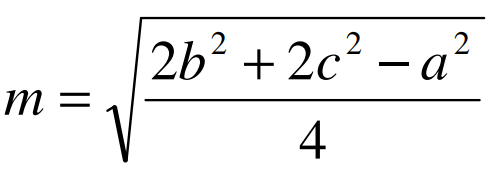
\includegraphics[width=0.6\linewidth]{source/5-maths/Temporary/Geometry-lingkaranSinggungSegitiga.png}
\end{multicols}

\textbf{Titik ke Garis}
\begin{verbatim}
U = ((x3-x1)(x2-x1)+(y3-y1)(y2-y1))/((x2-x1)^2+(y2-y1)^2)
X = x1 + U(x2-x1)
Y = y1 + U(y2-y1)
\end{verbatim}

\begin{multicols}{2}
\textbf{Dalil Steward} \\
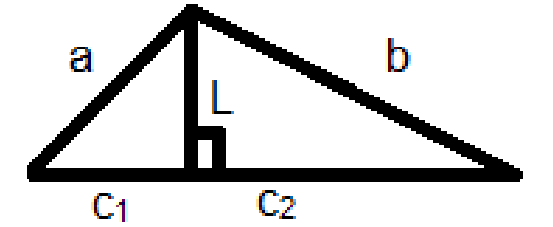
\includegraphics[width=0.5\linewidth]{source/5-maths/Temporary/Geometry-dalilSteward.png} \\
$L^2 . c = a^2.c_2 + b^2.c_1 - c_1.c_2.c$
\vfill\null\columnbreak
\textbf{Dalil Proyeksi} \\
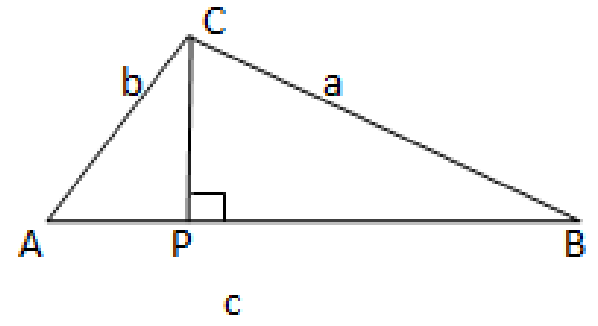
\includegraphics[width=0.5\linewidth]{source/5-maths/Temporary/Geometry-dalilProyeksi.png} \\
$AP = ( b^2 + c^2 - a^2 ) / 2c$
\end{multicols}

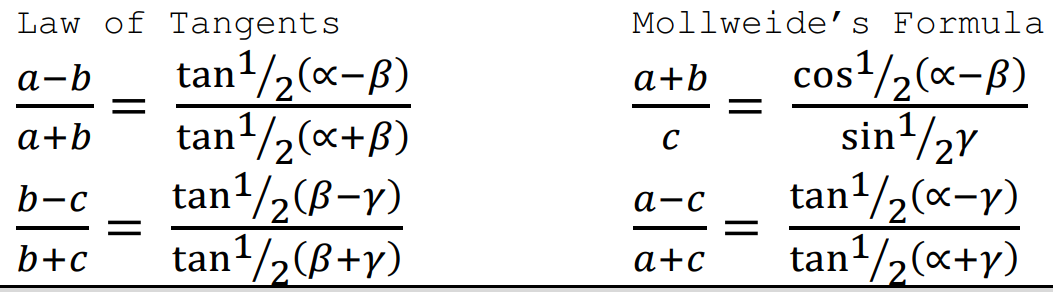
\includegraphics[width=0.8\linewidth]{source/5-maths/Temporary/Geometry-lawOfTangents.png}
